\documentclass[a4paper]{article}
\usepackage[utf8x]{inputenc}
\usepackage[T1,T2A]{fontenc}
\usepackage[russian]{babel}
\usepackage{hyperref}
\usepackage{indentfirst}
\usepackage{listings}
\usepackage{color}
\usepackage{here}
\usepackage{array}
\usepackage{multirow}
\usepackage{graphicx}

\usepackage{caption}
\renewcommand{\lstlistingname}{Программа} % заголовок листингов кода

\usepackage{listings}
\lstset{ %
extendedchars=\true,
keepspaces=true,
language=bash,					% choose the language of the code
basicstyle=\footnotesize,		% the size of the fonts that are used for the code
numbers=left,					% where to put the line-numbers
numberstyle=\footnotesize,		% the size of the fonts that are used for the line-numbers
stepnumber=1,					% the step between two line-numbers. If it is 1 each line will be numbered
numbersep=5pt,					% how far the line-numbers are from the code
backgroundcolor=\color{white},	% choose the background color. You must add \usepackage{color}
showspaces=false				% show spaces adding particular underscores
showstringspaces=false,			% underline spaces within strings
showtabs=false,					% show tabs within strings adding particular underscores
frame=single,           		% adds a frame around the code
tabsize=2,						% sets default tabsize to 2 spaces
captionpos=b,					% sets the caption-position to bottom
breaklines=true,				% sets automatic line breaking
breakatwhitespace=false,		% sets if automatic breaks should only happen at whitespace
escapeinside={\%*}{*)},			% if you want to add a comment within your code
postbreak=\raisebox{0ex}[0ex][0ex]{\ensuremath{\color{red}\hookrightarrow\space}}
}

\usepackage[left=2cm,right=2cm,
top=2cm,bottom=2cm,bindingoffset=0cm]{geometry}

\begin{document}	% начало документа

\begin{titlepage}	% начало титульной страницы

	\begin{center}		% выравнивание по центру

		\large Санкт-Петербургский Политехнический Университет Петра Великого\\
		\large Институт компьютерных наук и технологий \\
		\large Кафедра компьютерных систем и программных технологий\\[2cm]
		% название института, затем отступ 6см
		
		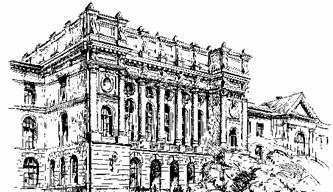
\includegraphics[scale=0.7]{pics/spbpu.jpg}\\[2cm]
		
		\huge Программирование\\[0.5cm] % название работы, затем отступ 0,5см
		\large Отчет по курсовой работе \\[0.1cm]
		\large Приложение "Sun Radio"\\[5cm]

	\end{center}


	\begin{flushright} % выравнивание по правому краю
		\begin{minipage}{0.25\textwidth} % врезка в половину ширины текста
			\begin{flushleft} % выровнять её содержимое по левому краю

				\large\textbf{Работу выполнила:}\\
				\large Кремнева ~В.Э.\\
				\large {Группа:} 23501/4\\
				
				\large \textbf{Преподаватель:}\\
				\large Вылегжанина ~К.Д.

			\end{flushleft}
		\end{minipage}
	\end{flushright}
	
	\vfill % заполнить всё доступное ниже пространство

	\begin{center}
	\large Санкт-Петербург\\
	\large \the\year % вывести дату
	\end{center} % закончить выравнивание по центру

\thispagestyle{empty} % не нумеровать страницу
\end{titlepage} % конец титульной страницы

\vfill % заполнить всё доступное ниже пространство








% Содержание
\tableofcontents
\newpage



\section{Проектирование приложения}

В современном мире музыка является неотъемлемой частью жизни многих и многих людей. Музыка часто сопровождает нас на работе, в дороге, во время досуга. Порой музыка может играть долгие часы. Настолько долгие, что за время прослушивания солнце может изменить свое положение относительно прослушивающего. Со временем суток так же меняется и настроение, и запас сил. И как было бы здорово, если бы музыка подстраивалась под наше самоощущение, дополняла и обогащала его.

\subsection{Задание}

Разработать приложение, позволяющее пользователям автоматически изменять тональность и громкость воспроизводимой музыки в соответствии с уровнем освещения.

\subsection{Концепция}

Изменения в музыкальные файлы вносятся с помощью преобразования Фурье. Информация об освещенности поступает с фоторезистра.

\subsection{Минимально работоспособный продукт}

Консольное приложение, получающее на вход музыкальный файл и воспроизводящее его в соответствии с текущим уровнем освещенности.

\subsection{Решаемые задачи}

В процессе проектирования приложения было выделено три основных задачи.

\begin{itemize}

\item \textbf{Получение спектра файла}

Для удобства работы используются .wav файлы. Удобство в том, что в каждом фрейме хранятся значения амплитуд, то есть имеем зависимость амплитуды от времени, что является входными данными для преобразования Фурье. С помощью этого преобразования получим спектр файла -- зависимость амплитуды от частоты. Но не всё так просто. При последовательном чтении фреймов накапливаются ошибки, поэтому необходимо использовать оконную функцию и читать данные с перекрытием. Эмпирически получено наилучшее перекрытие -- в одну шестнадцатую от количества читаемых фреймов при условии, что читаем по 2048 фреймов. Число фреймов, равное степени двойки, выбрано не случайно: это задел на будущее. Для быстрого преобразования Фурье необходимо число фреймов, равное степени двойки. Используемая оконная функция  -- функция Блэкмана-Наталла. Выбрана она за минимальный размер боковых лепестков и удовлетворительное "растяжение" спектра. При использовании входного фильтра необходим выходной фильтр. Выходной фильтр должен быть таким, чтобы сумма произведений входного и выходного фильтров в каждой точке была равна единице. Для этого здесь я просто нормализую входную оконную функцию.

\item \textbf{Корректные преобразования}

Необходимо изменить тон и громкость воспроизведения. Для изменения тона необходимо растянуть файл в N раз, интерполируя значения амплитуды и фазы между точками, а затем ускорить воспроизведение в N раз. Таким образом получим изменение тона при сохранении скорости воспроизведения.

\item \textbf{Воспроизведение файла}

Воспроизведение файла производится средствами javax.sound.sampled.*

\end{itemize}

\subsection{Выводы}

В данном разделе рассмотрен процесс проектирования приложения для модуляции звука в зависимости от уровня освещенности. Выделены основные задачи и предложены варианты их решения. 

\section{Реализация приложения}

\subsection{Среда разработки}

Операционная система: Windows 8.1

Среда разработки: IntelliJ IDEA 2016.3.4

Компилятор: javac, \verb|JDK 1.8.0_102|

\subsection{Выделенные классы}

В приложении были выделены следующие классы:
\begin{itemize}

\item \textbf{SunRadio}  - главный класс. Осуществляет основную работу приложения.

\item \textbf{Complex}  - класс для работы с комплексными числами. Взят из открытого источника.

\item \textbf{WavFile} - класс для работы с .wav файлами. Взят из открытого источника.

\item \textbf{WavFileException} - исключения для класса WavFile. Взят из открытого источника.

\item \textbf{LightLevel} - класс, с помощью которого можно получить текущий уровень освещенности.

\item \textbf{AM} - класс, содержащий средства для амплитудной модуляции. 

\item \textbf{DFTStraight} - реализует прямое дискретное преобразование Фурье. 

\item \textbf{DFTInverse} - реализует обратное дискретное преобразование Фурье. 

\item \textbf{Filter} - реализует оконную функцию.

\item \textbf{Interpolation} - реализует линецную интерполяцию по двум точкам.

\item \textbf{Scale} - реализует масштабирование в заданных пределах.   

\item \textbf{ToneModulation} - реализует модуляцию тона. 

\item \textbf{ToneModulationException} - исключения для класса ToneModulation. 

\end{itemize}

\subsection{Выводы}

В данном разделе были описаны все классы, выделенные в процессе работы над проектом.

\section{Процесс обеспечения качества и тестирование}

\subsection{Тестирование}

Для проверки работы библиотеки использовались автоматические тесты, покрывающие основную функциональность ядра. Также в процессе разработки приложения проводилось ручное тестирование программы.

\subsection{Выводы}

В данном разделе описан процесс тестирования программы. 

\section{Выводы}

В результате работы над курсовым проектом было реализовано приложение, предназначенное для изменения музыки в соответствии с уровнем освещенности. Изучено: преобразование Фурье, оконные функции, амплитудная модуляция, линейная интерполяция. Так же приобретены навыки разработки приложения на языке Java, а также навыки разработки тестов на языке Groovy.

\section{Приложение 1}

\captionof{lstlisting}{Complex.java}
\lstinputlisting{C:/Users/LEV/IdeaProjects/SunRadioo/src/com/external/Complex.java}
\parindent=1cm

\captionof{lstlisting}{WavFile.java}
\lstinputlisting{C:/Users/LEV/IdeaProjects/SunRadioo/src/com/external/WavFile.java}
\parindent=1cm

\captionof{lstlisting}{WavFileException.java}
\lstinputlisting{C:/Users/LEV/IdeaProjects/SunRadioo/src/com/external/WavFileException.java}
\parindent=1cm

\captionof{lstlisting}{LightLevel.java}
\lstinputlisting{C:/Users/LEV/IdeaProjects/SunRadioo/src/com/sunradio/core/LightLevel.java}
\parindent=1cm

\captionof{lstlisting}{SunRadio.java}
\lstinputlisting{C:/Users/LEV/IdeaProjects/SunRadioo/src/com/sunradio/core/SunRadio.java}
\parindent=1cm

\captionof{lstlisting}{AM.java}
\lstinputlisting{C:/Users/LEV/IdeaProjects/SunRadioo/src/com/sunradio/math/AM.java}
\parindent=1cm

\captionof{lstlisting}{DFTStraight.java}
\lstinputlisting{C:/Users/LEV/IdeaProjects/SunRadioo/src/com/sunradio/math/DFTStraight.java}
\parindent=1cm

\captionof{lstlisting}{DFTInverse.java}
\lstinputlisting{C:/Users/LEV/IdeaProjects/SunRadioo/src/com/sunradio/math/DFTInverse.java}
\parindent=1cm

\captionof{lstlisting}{Filter.java}
\lstinputlisting{C:/Users/LEV/IdeaProjects/SunRadioo/src/com/sunradio/math/Filter.java}
\parindent=1cm

\captionof{lstlisting}{Interpolation.java}
\lstinputlisting{C:/Users/LEV/IdeaProjects/SunRadioo/src/com/sunradio/math/Interpolation.java}
\parindent=1cm

\captionof{lstlisting}{Scale.java}
\lstinputlisting{C:/Users/LEV/IdeaProjects/SunRadioo/src/com/sunradio/math/Scale.java}
\parindent=1cm

\captionof{lstlisting}{ToneModulation.java}
\lstinputlisting{C:/Users/LEV/IdeaProjects/SunRadioo/src/com/sunradio/math/ToneModulation.java}
\parindent=1cm

\captionof{lstlisting}{ToneModulationException.java}
\lstinputlisting{C:/Users/LEV/IdeaProjects/SunRadioo/src/com/sunradio/math/ToneModulationException.java}
\parindent=1cm

\captionof{lstlisting}{SunRadioTest.groovy}
\lstinputlisting{C:/Users/LEV/IdeaProjects/SunRadioo/Test/com/sunradio/core/SunRadioTest.groovy}
\parindent=1cm

\captionof{lstlisting}{DFTStraightTest.groovy}
\lstinputlisting{C:/Users/LEV/IdeaProjects/SunRadioo/Test/com/sunradio/math/DFTStraightTest.groovy}
\parindent=1cm

\captionof{lstlisting}{DFTInverseTest.groovy}
\lstinputlisting{C:/Users/LEV/IdeaProjects/SunRadioo/Test/com/sunradio/math/DFTInverseTest.groovy}
\parindent=1cm

\captionof{lstlisting}{FilterTest.groovy}
\lstinputlisting{C:/Users/LEV/IdeaProjects/SunRadioo/Test/com/sunradio/math/FilterTest.groovy}
\parindent=1cm

\captionof{lstlisting}{ScaleTest.groovy}
\lstinputlisting{C:/Users/LEV/IdeaProjects/SunRadioo/Test/com/sunradio/math/ScaleTest.groovy}
\parindent=1cm

\end{document}